% ****** Start of file aipsamp.tex ******
%
%   This file is part of the AIP files in the AIP distribution for REVTeX 4.
%   Version 4.1 of REVTeX, October 2009
%
%   Copyright (c) 2009 American Institute of Physics.
%
%   See the AIP README file for restrictions and more information.
%
% TeX'ing this file requires that you have AMS-LaTeX 2.0 installed
% as well as the rest of the prerequisites for REVTeX 4.1
%
% It also requires running BibTeX. The commands are as follows:
%
%  1)  latex  aipsamp
%  2)  bibtex aipsamp
%  3)  latex  aipsamp
%  4)  latex  aipsamp
%
% Use this file as a source of example code for your aip document.
% Use the file aiptemplate.tex as a template for your document.
\documentclass[%
 aip,
 jmp,%
 amsmath,amssymb,
%preprint,%
reprint,%
%author-year,%
%author-numerical,%
]{revtex4-1}

\usepackage[title]{appendix}
\usepackage{dsfont}
\usepackage{tikz}
\usetikzlibrary{shapes,arrows}
%\usepackage{caption}
\usepackage{makecell}
\usepackage{graphicx}% Include figure files
\usepackage{dcolumn}% Align table columns on decimal point
\usepackage{bm}% bold math
%\usepackage[mathlines]{lineno}% Enable numbering of text and display math
%\linenumbers\relax % Commence numbering lines
\setlength{\parindent}{0.5cm}
\usepackage{natbib}
\setcitestyle{square}
\bibliographystyle{jcp}%{jcp}%{achemso}

\usepackage{bibentry}

\usepackage{mathtools}
\DeclarePairedDelimiter\ceil{\lceil}{\rceil}
\DeclarePairedDelimiter\floor{\lfloor}{\rfloor}

\definecolor{basilgreen}{rgb}{0.25, 0.42, 0.11}

\begin{document}

%\preprint{AIP/123-QED}

\title[Multi-state instantons]{On the multi-state instanton}% Force line breaks with \\
%\thanks{Footnote to title of article.}

\author{Srinath Ranya}
 \affiliation{Department of Chemistry and Chemical Biology, Cornell University}%Lines break automatically or can be forced with \\
\author{Nandini Ananth}%
 \email{ananth@cornell.edu.}
\affiliation{Department of Chemistry and Chemical Biology, Cornell University}
%Authors' institution and/or address%\\This line break forced with \textbackslash\textbackslash
%}%

%\author{C. Author}
% \homepage{http://www.Second.institution.edu/~Charlie.Author.}
%\affiliation{%
%Second institution and/or address%\\This line break forced% with \\
%}%

\date{\today}% It is always \today, today,
             %  but any date may be explicitly specified

\begin{abstract}
We determine the multi-state ring polymer instanton (MS-RPI) - an extension of the ring polymer instanton to multiple electronic states. The mean-field ring polymer instanton (MF-RPI) incorporates an average effect of the electronic states on the nuclear degree of freedom (DoF), whereas the coordinate mapping variable ring polymer (CMV-RPI) has explicit coordinate variables representing the electronic states. We analyze the MF-RPI and CMV-RPI in two state model systems coupled via a single nuclear mode over a range of driving forces, and in the adiabatic and non-adiabatic limits. *** Two sentences on key results ***
\end{abstract}

%\pacs{Valid PACS appear here}% PACS, the Physics and Astronomy
                             % Classification Scheme.
\keywords{Non-adiabatic instanton, mapping variables, ring polymer instanton}%Use showkeys class option if keyword
                              %display desired
\maketitle


%\begin{quotation}
%The ``lead paragraph'' is encapsulated with the \LaTeX\ 
%\verb+quotation+ environment and is formatted as a single paragraph before the first section heading. 
%(The \verb+quotation+ environment reverts to its usual meaning after the first sectioning command.) 
%Note that numbered references are allowed in the lead paragraph.
%
%The lead paragraph will only be found in an article being prepared for the journal \textit{Chaos}.
%\end{quotation}

\section{\label{sec:level1}INTRODUCTION}
The computation of reaction rate constants for a reaction proceeding on the ground electronic surface has been the focus of many articles and reviews\cite{Eyring1935}. The importance of incorporating tunneling effects was demonstrated early on\cite{Wigner1938}. Subsequent work has been directed towards determining a reaction rate theory which includes the quantum nature of systems\cite{Pechukas1981, Truhlar1983, Pollak2005,Chapman1975, Hele2013, Richardson2017}. \par
Quantum mechanical tunneling is incorporated using the instanton - a periodic orbit on the inverted potential energy surface (PES) - in semiclassical instanton (SCI) theory\cite{Chapman1975}. However, the determination of these periodic orbits is a trajectory-search problem, which is no easy task. The ring polymer instanton (RPI) - a discrete approximation to the instanton - alleviates this difficulty by reformulating it as the search for a first order saddle point on the extended ring polymer (RP) PES\cite{Richardson2009}. Once the RPI is determined, the Im F premise is used to compute the rate. The Im F premise has been shown to be the steepest-descent limit of the flux-side formulation of SCI theory\cite{Althorpe2011}. 

The simulation of electron transfer and photo-initiated processes are harder because they are non-adiabatic by nature\cite{Marcus1985, Sutin2007, Gray1996}.  Semiclassical (SC)\cite{Topaler1996, Neria1993} and trajectory-hopping\cite{Tully1990} methods to determine their rates have been developed and tested on model and simple systems. Others have given compact expressions for the rate constants by combining SCI theory with the Zhu-Nakamura transition formulae\cite{Teranishi2012}. Instanton trajectory methods that require a self-consistent evaluation of the electronic wavefunctions and the nuclear trajectory, have been shown to work in the low-temperature regime\cite{Cao1995, Cao1997, Jang2001} for a range of coupling regimes.  Working in the adiabatic basis requires the computation of non-adiabatic coupling vectors which can be unpleasant if the system has conical intersections\cite{Yarkony1996}, thus motivating the diabatic representation. 

Working in the diabatic basis, the Stock-Thoss (ST) mapping protocol\cite{Stock1997} can be used to introduce continuous variables for  electronic DoFs, allowing them to be treated on the same dynamical footing as the nuclei. Imaginary time dynamical methods such as mapping-variable ring polymer molecular dynamics (MV-RPMD)\cite{Ananth2013}, nonadiabatic RPMD\cite{Richardson2013}, coherent state RPMD\cite{Chowdhury2017} have shown promise towards the simulation of non-adiabatic dynamics. RPI methods in the non-adiabatic limit have also been studied\cite{Richardson2015a,Richardson2015b}. 

In this paper, we propose two multi-state (MS) RPIs: (a) the mean-field (MF) RPI (b) the coordinate mapping-variable (CMV) RPI and develop a computational methodology for their determination. We demonstrate the the CMV-RPI can accurately capture the physics as compared to the MF-RPI. The paper is organized is as follows: In Sec. \ref{sec:level2} we provide an overview of the MF-RPI and CMV-RPI approaches, followed a brief description of the model systems in Sec. \ref{sec:level3} while the implementation details are provided in Sec. \ref{sec:level4}. Sec. \ref{sec:level5} discusses the results, and conclusions are drawn in Sec. \ref{sec:level6}. 

\section{\label{sec:level2}THEORY}
The formalism is presented for a $\mathcal{K}$-state Hamiltonian with $f$ nuclear DoFs, in the diabatic representation:
\begin{eqnarray}
\hat{H}(\hat{\mathbf{R}},\hat{\mathbf{P}}) & \equiv & \dfrac{\hat{\mathbf{P}}^{T}\hat{\mathbf{P}}}{2M} + \mathbf{V}(\hat{\mathbf{R}})  \notag  \\
\mathbf{V}(\hat{\mathbf{R}})  & = & \sum_{n,m=1}^{\mathcal{K}} |\psi_{n} \rangle V_{nm}(\hat{\mathbf{R}}) \langle \psi_{m} |
\end{eqnarray} 
Here, $\hat{\mathbf{R}}$ and $\hat{\mathbf{P}}$ represent positions and momenta of the nuclear DoFs, and $\mathbf{V}(\hat{\mathbf{R}})$ is the diabatic matrix. $\{|\psi_{n}\rangle\}$ is the set of diabatic electronic states, $V_{nn}(\hat{\mathbf{R}})$ the diabatic potentials and $V_{nm}(\hat{\mathbf{R}})$ the coupling between the diabatic states $n,m$. The canonical partition function is obtained by computing the trace of the Boltzmann operator: 
\begin{eqnarray}
\mathcal{Z} & = & \mathrm{Tr}_{ne}[e^{-\beta\hat{H}}] \\
& \propto & \lim_{N\rightarrow \infty} \int d\{ \mathbf{R}_{\alpha} \} e^{-\beta U_{\mathrm{sp}}} \mathrm{Tr}_{e}\left[\prod_{\alpha=1}^{N} e^{-\beta_{N} \mathbf{V}(\mathbf{R}_{\alpha})}\right] \label{ZNElec}
\end{eqnarray}
Here, the subscripts $n$,$e$ denote that the trace is carried over the electronic and nuclear DoFs, respectively. $U_{\mathrm{sp}}$ arises from the inter-bead coupling through springs:
\begin{equation}
U_{\mathrm{sp}} = \dfrac{1}{N}\sum_{\alpha} \dfrac{M}{2\beta_{N}^2}(\mathbf{R}_{\alpha} - \mathbf{R}_{\alpha+1})^T(\mathbf{R}_{\alpha} - \mathbf{R}_{\alpha+1})
\end{equation}
The trace over the nuclear DoFs is evaluated in the $f$-dimensional position $\mathbf{R}$ representation; however, there are multiple choices when it comes to the electronic DoFs. It is this freedom that allows us to formulate two RPIs for the MS system.
\subsection{\label{ssec:level2A} MF PI representation of the partition function}
The introduction of $N$ copies of the resolution of identity in the diabatic basis
\begin{equation}
\mathds{1} = \sum_{n} | \psi_{n} \rangle \langle \psi_{n} |
\end{equation}
allows for the evaluation of the trace over the electronic coordinates yielding:
\begin{eqnarray}
\mathrm{Tr}_{e}\left[\prod_{\alpha=1}^{N} e^{-\beta_{N} \mathbf{V}(\mathbf{R}_{\alpha})}\right] & = & \mathrm{Tr}\left[ \prod_{\alpha=1}^{N} \mathcal{M}(\mathbf{R}_{\alpha},\mathbf{R}_{\alpha+1})\right]  \label{gamma} 
\end{eqnarray}
where the matrix elements of $\mathcal{M}(\mathbf{R}_{\alpha},\mathbf{R}_{\alpha+1})$ are evaluated in the high-temperature limit using the symmetric Trotter expansion. 
%\begin{widetext}
\begin{eqnarray}
\mathcal{M}_{nn} & = & e^{-\beta_{N}[V_{nn}(\mathbf{R}_{\alpha})+V_{nn}(\mathbf{R}_{\alpha})]} \notag \\
\mathcal{M}_{nm} & = & -\beta_{4N}  \left[  \makecell{V_{nm}(\mathbf{R}_{\alpha}) + V_{nm}(\mathbf{R}_{\alpha+1}) } \right] \notag \\ & \times & \left[ \makecell{e^{-\beta_{N}[V_{nn}(\mathbf{R}_{\alpha})+V_{nn}(\mathbf{R}_{\alpha+1})]} \vspace*{0.2cm}\\ + e^{-\beta_{N}[V_{mm}(\mathbf{R}_{\alpha})+V_{mm}(\mathbf{R}_{\alpha+1})]} } \right] 
\end{eqnarray} 
%\end{widetext}
The canonical partition function in the MF representation is given by:
\begin{eqnarray}
\mathcal{Z}_\mathrm{MF} & \propto & \lim_{N\rightarrow \infty} \int d\{ \mathbf{R}_{\alpha} \} e^{-\beta V_{\mathrm{MF}}(\{ \mathbf{R}_{\alpha} \})} \mathrm{sgn}(\Gamma_{\mathrm{MF}})
\end{eqnarray}
The extended RP potential $V_{\mathrm{MF}}(\{ \mathbf{R}_{\alpha} \})$ is given by:
\begin{eqnarray}
V_{\mathrm{MF}}(\{ \mathbf{R}_{\alpha} \}) = U_{\mathrm{sp}} - \dfrac{1}{\beta} \ln | \mathrm{Re}(\Gamma_{\mathrm{MF}}) |
\end{eqnarray}
where $\Gamma_{\mathrm{MF}}$ is given by Eq. \eqref{gamma}, and comprises of the interactions amongst electronic states of all beads . 

\subsection{\label{ssec:level2B} CMV PI representation of the partition function}
The ST mapping protocol maps the $\mathcal{K}$ diabatic electronic states onto states in the singly excited oscillator (SEO) subspace of $\mathcal{K}$ harmonic oscillators. 
\begin{eqnarray}
| \psi_{n} \rangle \langle \psi_{m} |  & \rightarrow & \hat{a}_{n}^{\dagger}\hat{a}_{m} \notag\\
| \psi_{n} \rangle & \rightarrow & | 0_{1},\dots,1_{n},\dots,0_{\mathcal{K}}\rangle \equiv | n\rangle 
\end{eqnarray}
where $|n\rangle$ denotes that the $n^{\mathrm{th}}$ oscillator is in the first excited state. The resolution of identity in the electronic coordinate ($\mathbf{x}$) representation in this SEO space is given by:
\begin{equation}
\mathds{1} = \int d\mathbf{x} \mathcal{P} |\mathbf{x}\rangle \langle \mathbf{x}| \mathcal{P}
\end{equation}
where the projection operator $\mathcal{P} = \sum_{n} | n \rangle \langle n |$ constrains the electronic coordinates to the SEO subspace. 
Introducing $N$ copies of the identity in Eq. \eqref{ZNElec} to evaluate the trace over electronic states, we obtain:
\begin{eqnarray}
\mathcal{Z}_{\mathrm{CMV}} & \propto & \lim_{N\rightarrow \infty} \int d\{ \mathbf{R}_{\alpha} \}  \int d\{ \mathbf{x}_{\alpha} \} e^{-\beta U_{\mathrm{sp}}} e^{-\sum_{\alpha}\mathbf{x}_{\alpha}^T\mathbf{x}_{\alpha}}\notag \\
& \times & \mathrm{Tr}\left[ \prod_{\alpha=1}^{N} \mathcal{X}_{\alpha} \mathcal{M}(\mathbf{R}_{\alpha},\mathbf{R}_{\alpha+1}) \right] \label{gammaCMV}
\end{eqnarray}
The matrix elements of $\mathcal{X}_{\alpha} = \mathbf{x}_{\alpha} \otimes \mathbf{x}_{\alpha}^{T}$, the electronic matrix, are evaluated using the SEO wave functions:
\begin{eqnarray}
\langle \mathbf{x} | n \rangle  = \dfrac{\sqrt{2}}{\pi^{\mathcal{K}/4}} [\mathbf{x}]_{n} e^{-\frac{1}{2}\mathbf{x}^{T}\mathbf{x}}
\end{eqnarray}
Here, we note that this derivation closely follows that in Ref. \cite[23]{} and differs only in the evaluation of the matrix elements of the the $\mathcal{M}$ matrix. The CMV-PI representation of the partition function, and the extended CMV-PES ($V_{\mathrm{CMV}}$) is given by:
\begin{eqnarray}
\mathcal{Z}_{\mathrm{CMV}} & \propto & \lim_{N\rightarrow \infty} \int d\{ \mathbf{R}_{\alpha} \}  \int d\{ \mathbf{x}_{\alpha} \} e^{-\beta V_{\mathrm{CMV}}} \mathrm{sgn}(\Gamma_{\mathrm{CMV}})\notag \\
V_{\mathrm{CMV}} & = & U_{\mathrm{sp}} + \dfrac{1}{\beta} \sum_{\alpha}\mathbf{x}_{\alpha}^T\mathbf{x}_{\alpha} - \dfrac{1}{\beta} \ln | \mathrm{Re}(\Gamma_{\mathrm{CMV}}) |
\end{eqnarray}
where $\Gamma_{\mathrm{CMV}}$ is the trace over the product of the $\mathcal{X}$ and $\mathcal{M}$ matrices for all beads, as shown in Eq. \eqref{gammaCMV}

\subsection{\label{ssec:level2C} Determination of the RPIs}
The RPI configuration is the first order saddle point on the extended RP-PES\cite{Richardson2009}. We hypothesize that this must hold true even for the case of multiple electronic states. Therefore, the MF-RPI must satisfy the following $fN$ equations given by the extremization of $V_{\mathrm{MF}}$, i.e., 
\begin{equation}
\frac{\partial V_{\mathrm{MF}}}{\partial [\mathbf{R}_{\alpha}]_{i}} = 0 
\end{equation}
The CMV-RPI satisfies $(f+\mathcal{K})N$ equations simultaneously, obtained by extremizing $V_{\mathrm{CMV}}$, i.e.,
\begin{eqnarray}
\frac{\partial V_{\mathrm{CMV}}}{\partial [\mathbf{R}_{\alpha}]_{i}} & = & 0  \\
\frac{\partial V_{\mathrm{CMV}}}{\partial [\mathbf{x}_{\alpha}]_{j}} & = & 0 
\end{eqnarray}
where $\alpha=1,\dots,N$ runs over the bead indices; $i=1,\dots,f$ and $j=1,\dots, \mathcal{K}$ represent the dimensionality of the nuclear and electronic DoFs.
\subsection{\label{ssec:level2D} Zero mode of the instanton}
An instanton solution is invariant to imaginary time translation. Equivalently, in the RP representation - the instanton configuration is invariant to permutation of the beads. The action for a periodic orbit on the inverted potential is given by:
\begin{eqnarray}
\mathcal{S}_{\mathrm{MS}}  = && \int_{0}^{\beta} d\tau \left[ \dfrac{M}{2}\left( \dfrac{d \mathbf{X}(\tau)}{d\tau}\right)^2 + \mathrm{V_{MS}}[\mathbf{X}(\tau)]\right] 
\end{eqnarray}
The equation of motion for the periodic orbit is an extremum of the first variation of the action ($\delta \mathcal{S}_{\mathrm{MS}} = 0$) 
\begin{eqnarray}
- M \dfrac{d^2 \mathbf{X}(\tau)}{d\tau^2} + \nabla_{\mathbf{X}} \mathrm{V_{MS}}[\mathbf{X}(\tau)] = 0 \label{ms-eom} 
\end{eqnarray}
and the second variation $\delta^2 \mathcal{S}_{\mathrm{MF}}$ gives us the stability matrix $\tilde{\mathbf{S}}_{\mathrm{MS}}$ which describes the nature of the periodic orbit. Differentiating Eq. \eqref{ms-eom} w.r.t. $\tau$, we obtain:
\begin{eqnarray}
&& \dfrac{d}{d\tau} \left[ - M \dfrac{d^2 \mathbf{X}(\tau)}{d\tau^2} + \nabla_{\mathbf{X}}\mathrm{V_{MS}}  \right] =   \tilde{\mathbf{S}}_{\mathrm{MS}}\dot{\mathbf{X}}(\tau) = 0 \times \dot{\mathbf{X}}(\tau) \notag \\
\end{eqnarray}
The velocity mode, where $\mathbf{X}$ represents all the DoFs, turns out to be the zero mode. A more elaborate derivation, and the specific structure of the stability matrices in the MF and CMV cases can be found in Appendices \ref{sec:AppendA} and \ref{sec:AppendB}, respectively. 

\section{\label{sec:level3} MODEL SYSTEMS}
We consider three models: two-state ($\mathcal{K}=2$) systems coupled by one nuclear DoF ($f=1$) represented by the Hamiltonian 
\begin{equation}
\hat{H}(\hat{R},\hat{P}) = \dfrac{\hat{P}^2}{2M} + \mathbf{V}(\hat{R})
\end{equation}
Here, $\mathbf{V}(R)$ is the diabatic potential matrix, whose diagonal elements are given by:
\begin{eqnarray}
V_{ii}(R) & = & \dfrac{1}{2} M \omega^2 (R-R_{i})^2 + \epsilon \delta_{1i} 
\end{eqnarray}
which represent electron donor and acceptor states, and the off-diagonal terms ($V_{12} = \Delta$) - the coupling between them. The nuclear mass $(M)$ and the frequency $(\omega)$ of the oscillators is set to $2\ a.u.$, and to $1\ a.u.$, respectively. 

The models are shown in Fig.~\ref{fig:DApot}
\begin{figure}[h!]
\centering
%\includegraphics[scale=0.3]{model-pes.png}
\includegraphics[scale=0.16]{model-pot-6.png}%-green.png}%2.png} 
\caption{Red (dot-dashed) and grey (continuous) lines show the donor and acceptor states in Model I (symmetric system); the green (dashed) and black (dotted) lines represent the donor state in Models II and III which are asymmetric systems with $\epsilon=10.0$ and $20.0$, respectively. $R_{1}$ and $R_{2}$ represent the minima of the donor and acceptor states and $R_{0}$ marks the crossing in Model I.} \label{fig:DApot}
\end{figure}
and differ in the driving force difference between the donor and acceptor states with $\epsilon=0.0,10.0,20.0$ for the three models. They are studied over a range of temperatures, in the adiabatic (strong coupling) and non-adiabatic (weak coupling) limits. For the temperatures considered, the coupling between the donor and acceptor states is chosen such that $\Delta/k_{B}T=2.0$ and $0.025$ in the adiabatic and non-adiabatic limits, respectively. The specific values of coupling are given in Table. \ref{CouplingTable}
\\
\begin{table}[ht!]
\renewcommand{\arraystretch}{1.25}
\begin{tabular}{|c|c|c|} \hline
$\beta$& $ \mathbf{\Delta} $ & $\Delta$ \\ \hline % _{\mathrm{adiabatic}}$ & $\Delta_{\mathrm{non-adiabatic}}$ \\ \hline
2.5 & \textbf{0.8}  & 0.01 \\ %\hline
2.0 & \textbf{1.0} & 0.0125\\ %\hline
1.75 & \textbf{1.143}  & 0.0143 \\ %\hline
1.5 & \textbf{1.333} & 0.0166 \\ %\hline
1.4 & \textbf{1.429} & 0.0179\\ \hline
\end{tabular}
\caption{The coupling for different temperatures in the adiabatic (in bold) and non-adiabatic limits such that $\beta\mathbf{\Delta}=2.0$ and $\beta\Delta = 0.025$} \label{CouplingTable}
\renewcommand{\arraystretch}{1}
\end{table}
%We study electron donor-acceptor systems in the adiabatic and non-adiabatic limits, over a range of driving forces, coupling strength, and system temperatures. We model the donor and acceptor states using harmonic oscillators; the nuclear DoF coupling them is treated quantum mechanically. In the adiabatic and non-adiabatic limits, we choose $\beta$ and $\Delta$ such that $\beta\Delta = 2.0$ and $0.025$, respectively. 

\section{\label{sec:level4} IMPLEMENTATION DETAILS}
\subsection{\label{ssec:level4A} Initial guess for the nuclear and electronic coordinates}

For a RP with $N$ beads, two beads are fixed to the crossing, and $N_{1}$ and $N_{2}$ beads are initialized to the donor and acceptor states. The constraining of two beads to the crossing is a necessity in the case of the system with a driving force, where the beads tend to fall to the acceptor minimum. 
A representative initial guess (IG) for the nuclear coordinates along with the corresponding IG for the electronic coordinates, for model II,  is shown in Fig. \ref{IGfig}.
\begin{figure}[h!]
\includegraphics[scale=0.16]{initGuess-128-44-84B-latest.png} \includegraphics[scale=0.16]{initGuess-pop-128-44-84B-2.png}
\caption{Plots of initial guesses for a 128-bead RP for Model II, and for the case $N_{1}=44,N_{2}=82$. Beads on the donor are colored green (squares), those on the acceptor - gray (cirles), and the ones constrained to the crossing in red. The dashed line represents the crossing of the two diabats. Also shown is the population of the donor state (Wigner estimator) in each bead, for the given nuclear IG.}\label{IGfig}
\end{figure}
The IG for the nuclear variables of the RP is obtained using the following expressions:
\begin{center}
{\color{gray} $ R_{0}+\left(R_{2}-R_{0}\right) \cos\left( \dfrac{\pi i }{N_{2}+1}\right) \mathrm{for}\ i=1, \floor*{\dfrac{N_{2}}{2}} $ } \vspace*{0.25cm}\\
{\color{green} $   R_{0} - \left| \left( R_{0} - R_{1} \right) \cos\left( \dfrac{\pi}{2} + \dfrac{\pi i }{N_{1}+1}\right) \right| \mathrm{for}\ i=1, N_{1} $ } \vspace*{0.25cm}\\
{\color{gray} $ R_{0}+\left(R_{2}-R_{0}\right) \cos\left( \dfrac{\pi i }{N_{2}+1}\right) \mathrm{for}\ i= \floor*{\dfrac{N_{2}}{2}}+2, N_{2} $ } 
\end{center} 
One bead is placed at the crossing after each separate segment, shown in different colors. These are used as input to RPI calculations on the lower adiabatic surface, and the resulting RPI coordinates are used to find reasonable IGs for the electronic coordinates:
\begin{eqnarray}
\left[\mathbf{x}_{\alpha}\right]_{n} & = & \sqrt{\dfrac{e^{-\beta V_{nn}(R_{\alpha})}}{\sum_{n} e^{-\beta V_{nn}(R_{\alpha})} }}
\end{eqnarray}
Please see flowchart for more details. 
\subsection{\label{ssec:level4B} Determination of the instanton}
The L-BFGS-B algorithm is used for optimization as it's update procedure preserves the index of the Hessian matrix, indicating that a reasonable initial guess might converge to the desired answer - the instanton. 
The ratio $N_{1}:N_{2}$ is varied and the extended MS-RP potential determined. A particular ratio of $N_{1}:N_{2}$ maximizes it; this configuration of the beads is the instanton configuration as shown in Fig. \ref{rppesN1N2} 
\begin{figure}[h!]
\centering
\includegraphics[scale=0.38]{MF-action.png} 
\caption{Plot of the RP potential as s function of the $N_{1}$} \label{rppesN1N2}
\end{figure}
To aid in the convergence of the high-dimensional CMV instanton calculations, the protocol described in Fig. \ref{fig:Protocol} was devised. Calculations are performed to determine the adiabatic and non-adiabatic single surface (SS) instantons which are used as inputs to the subsequent calculations. Further, the $N_{1}$ beads are constrained to the region between the minimum of the donor well $R_{1}$ and the point of crossing $R_{0}$, and the $N_{2}$ beads to the region between the crossing and the acceptor minimum $R_{2}$. This is particularly useful for calculations in models with a driving force where all the nuclear beads tend to move towards the acceptor state.
\begin{figure}[ht!]
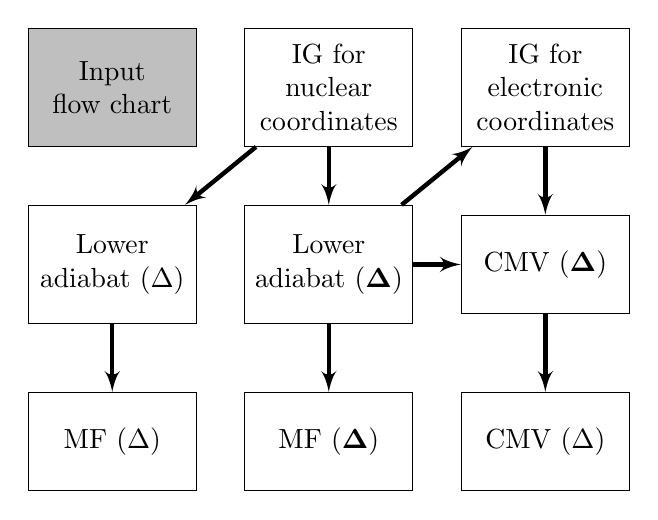
\begin{tikzpicture}[auto,line/.style={draw, ultra thick, -latex', shorten >= 0pt}]
\node [rectangle, draw=black, fill=white, text width=1.9cm, minimum height=1.5cm, text centered, anchor=center] (IG) {IG for \\ nuclear \\ coordinates}; 
\node [rectangle, draw=black, left of =IG, xshift=-1.75cm, fill=lightgray, text width=1.9cm, minimum height=1.5cm, text centered, anchor=center] (flowchart) {Input flow chart}; 
\node [rectangle, below of = IG, yshift=-1.25cm, draw=black,  fill=white, text width=1.9cm, minimum height=1.5cm, text centered] (AASS) { Lower adiabat ($\mathbf{\Delta}$)}; 
\node [rectangle, right of = IG, xshift=1.75cm, draw=black,  fill=white, text width=1.9cm, minimum height=1.5cm, text centered] (EECMV) {IG for \\ electronic \\ coordinates}; 
\node [rectangle, left of = AASS, xshift=-1.75cm, draw=black,  fill=white, text width=1.9cm, minimum height=1.5cm, text centered] (NASS) {Lower adiabat ($\Delta$)}; 
\node [rectangle,  below of = AASS, yshift=-1.25cm, draw=black,  fill=white, text width=1.9cm, minimum height=1.25cm, text centered] (AAMF) {MF ($\mathbf{\Delta}$)}; 
\node [rectangle,  below of = NASS, yshift=-1.25cm, draw=black,  fill=white, text width=1.9cm, minimum height=1.25cm, text centered] (NAMF) {MF  ($\Delta$)};
\node [rectangle, right of = AASS, xshift=1.75cm, draw=black,  fill=white, text width=1.9cm, minimum height=1.25cm, text centered] (AACMV) {CMV ($\mathbf{\Delta}$)};
\node [rectangle, below of = AACMV, yshift=-1.25cm, draw=black, fill=white, text width=1.9cm, minimum height=1.25cm, text centered] (NACMV) {CMV ($\Delta$)}; 

\begin{scope}[every path/.style=line]
  \path (IG) -- (AASS);
  \path (IG) -- (NASS);
  \path (AASS) -- (AAMF);
  \path (AASS) -- (EECMV);
  \path (AASS) -- (AACMV);
  \path (NASS) -- (NAMF);
  \path (EECMV) -- (AACMV);
  \path (AACMV) -- (NACMV);
\end{scope}
\end{tikzpicture}
\caption{Protocol to determine the non-adiabatic instanton. Here, the $\mathbf{\Delta}$ and $\Delta$ represent the strong and weak coupling limits, respectively. CMV and MF are as defined previously. } \label{fig:Protocol}
\end{figure}
\subsection{\label{ssec:level4C}Population estimators}
The Wigner population estimator for the $n^{th}$ state in the $\alpha^{th}$ bead 
\begin{eqnarray}
\mathbb{P}_{\alpha n} & = & \left[\mathbf{x}_{\alpha}\right]_{n}^2
\end{eqnarray}
Here, the average donor state population $\mathcal{P}_{1}$ is the bead average of the donor state populations of all beads:
\begin{equation}
\mathcal{P}_{n} = \dfrac{1}{N}\sum_{\alpha=1}^{N} \mathbb{P}_{\alpha,n} = \dfrac{1}{N}\sum_{\alpha=1}^{N}\left[\mathbf{x}_{\alpha}\right]_{n}^2
\end{equation}
\section{\label{sec:level5}RESULTS AND DISCUSSION}
%We present the RPIs in the different multi-state formulations, and analyze their behavior over a range of couplings varying from the strong to weak coupling limits, and over a range of temperatures provided in Table \ref{CouplingTable}. These parameters are chosen such that the key trends are made transparent. First, we describe the key result of the paper: the CMV instanton and it's behavior in the strong and weak coupling limits. 
\subsection{\label{ssec:level5A}The CMV instanton}
 The CMV instanton is a first-order saddle point on the $3N$ dimensional potential $V_{\mathrm{CMV}}$ where $N$ is the number of RP beads. The diagonalization of the hessian of the CMV-RP - yields $3N$ eigenvalues of which one is negative and another numerically zero, i.e., about 4-5 orders of magnitude smaller compared to the next immediate eigenvalue, indicating that we have an instanton solution which is invariant under the permutation of beads. Below, we discuss the CMV-RPIs in different parameter regimes, and present results supporting our claim. 
\subsubsection{\label{sssec:level5A1} The effect of coupling}
We present results for a $N=256$ bead RP at $\beta=1.5$ for Model I.  The plots of the nuclear beads and the donor state population are shown in Figs. \ref{fig:NAAIns} and \ref{fig:NAAPop}, respectively. 
\begin{figure}[ht!]
\centering
\includegraphics[scale=0.16]{MV-Adia-Non-adia-Ins-b15-symm.png}
\caption{Nuclear bead positions of the CMV instanton for model I at $\beta=1.5$ in the adiabatic (continuous line) and non-adiabtic (circles with line) limits. The crossing of the donor and acceptor diabats are represented using the horizontal line.} \label{fig:NAAIns}
\end{figure}
\begin{figure}[ht!]
\centering
\includegraphics[scale=0.16]{MV-Adia-Non-adia-Pop-b15-symm.png}
\caption{Donor state populations obtained using the CMV instanton computed for Model I at $\beta=1.5$ in the adiabatic (continuous line) and non-adiabatic (circles with line) limits. } \label{fig:NAAPop}
\end{figure}
The spread of the nuclear beads is seen to be larger in the weak coupling limit compared to that in the strong coupling limit. This is in keeping with the fact that the curvature of the barrier in the latter case is larger than in former. The population of the donor state follows the nuclear beads in both cases. In the strong coupling limit, there is a finite population in the donor state even when the bead is away from the point of crossing; a "collapse" of electronic state character to the acceptor state is seen as it approaches the crossing and crosses over to the donor state. Moving further away, there is a drop in the donor state population which indicates that the donor and acceptor states are entangled due to the strong coupling. In the weak coupling limit, the influence of the acceptor state is visible only as the bead approaches the point of crossing. 
\par The eigenvalues obtained upon diagonalization of the hessian of the CMV-RP potential are plotted in Fig. \ref{fig:EigValCMV}

\subsubsection{\label{sssec:level5A2} The effect of the driving force}
The CMV instanton is determined for Models I, II and III using $256$ beads and at $\beta=1.5$, in the strong coupling limit. 
\begin{figure}[ht!]
\centering
\includegraphics[scale=0.16]{MV-Adia-Ins-b15-shifted2.png}
\caption{Plot of nuclear bead positions of the CMV instanton for different driving forces at $\beta=1.5$, in the adiabatic limit. Dot-dashed (red), dashed (green), and dotted (black) lines are used to represent Models I, II, and II, respectively whereas the horizontal black line is indicative of the crossing of the two diabats. } \label{fig:AdiaInsAllModels}
\end{figure}
\begin{figure}[ht!]
\centering
\includegraphics[scale=0.16]{MV-Adia-Pop-b15-combined-lines2.png}
\caption{Donor state populations of the CMV instanton in the adiabatic limit at $\beta=1.5$ are shown. Red (innermost), green, and black(outermost) lines represent Models I, II, and III, respectively.  } \label{fig:DSPopAdiaCMV}
\end{figure}
The nuclear coordinates of the instantons for Models II and III have been shifted by $-0.5$ and $-1.0$ units, respectively, in Fig. \ref{fig:AdiaInsAllModels}. Thus, the crossing of the different models are all at $0.0$, and this allows for a straightforward comparison. The effect of the driving force is to shift nuclear beads from the acceptor state onto the donor state as it's energy is increased. Here, any bead to the left of the crossing is termed as a bead on the donor, and that to the right - on the acceptor, and is indicative of the state with a larger population on the individual bead. Here, too, we observe the "collapse" effect, described in the previous section, indicating that the electronic populations are governed by nuclear bead positions and the coupling between the states. 
\begin{table}[ht!]
\renewcommand{\arraystretch}{1.5}
\centering
\begin{tabular}{|c|c|c|c|c|c|c|c|c|c|} \hline
\multicolumn{4}{|c|}{} & \multicolumn{3}{c|}{Adiabatic}     & \multicolumn{3}{c|}{Non-adiabatic}  \\ \hline
$\epsilon$ & $N_{1}$ & $N_{2}$& $R_{0}$ & $\bar{R}$ & $\mathcal{P}_{1}$ & $\mathcal{P}_{2}$ & $\bar{R}$ & $\mathcal{P}_{1}$ & $\mathcal{P}_{2}$ \\ \hline
0.0 & 63 & 63 & 0.0 & $ 10^{-6}$ & 0.50  & 0.50 & $ 10^{-6}$ & 0.50  & 0.50    \\ \hline
10.0 & 71 & 55 & -0.5 & -0.553  & 0.562 & 0.438 & -0.557  & 0.564  &  0.436 \\ \hline
20.0 & 79 & 47 &  -1.0 &  -1.100 & 0.623 & 0.377 &  -1.110  &  0.628   & 0.372  \\ \hline
\end{tabular}
\caption{Results for the CMV instanton are tabulated here. The nuclear centroid $(\bar{R})$, average donor and acceptor state populations and the ratio of beads on donor and acceptor surfaces, in the adiabatic and non-adiabatic limits, at $\beta=1.5$} \label{table:CMV}
\renewcommand{\arraystretch}{1.0}
\end{table}
The effect of the coupling strength on the CMV-RPI for the model systems is tabulated in Table. \ref{table:CMV}. It shows that the number of beads that shift from the acceptor to the donor is proportional to the driving force, i.e., the ratio $N_{1}/N_{2}$ increases linearly with the driving force, and is independent of the coupling strength. 

\subsection{\label{ssec:level5B} Comparison of the SS, MF and CMV instantons}
The effect of the various parameters on the RPIs are analyzed for model I. The single surface instanton determined at different temperatures is plotted in Fig. \ref{fig:ins}; these computations are in the adiabatic regime of coupling. It is observed that the spread of the RP reduces as we increase the temperature, and will eventually collapse to the crossing point at the crossover temperature. 
%\begin{center}%
\begin{figure}[ht!]
\centering
%\includegraphics[scale=0.35]{adia-instanton.png}
%\includegraphics[scale=0.16]{adia-instanton3.png}
\includegraphics[scale=0.16]{adia-instantons-lines.png}
%\includegraphics[scale=0.2]{adia-instanton.png}\includegraphics[scale=0.2]{Nadia-instanton.png} \\
%\includegraphics[scale=0.2]{MVadia-instanton.png} \\
%\includegraphics[scale=0.2]{MVNadia-instanton.png}\includegraphics[scale=0.2]{instantons-125-256.png} 
%\includegraphics[scale=0.16]{figure-1B.png}\\
%\includegraphics[scale=0.16]{MVNadia-instanton2.png}
%\caption{256 beads were used for the calculations. We plot the instanton configuration as a function of the temperature - darker the color of blue, higher the temperature. Here, the sub-figures represent the following cases: (a) single surface instanton in the adiabatic limit, (b) single surface instanton in the non-adiabatic limit, (c) mean-field instanton in the adiabatic limit, (d) CMV instanton in the adiabatic limit, (e) CMV in the non-adiabatic limit}
\caption{The single surface instanton, in the adiabatic limit, is shown as a function of inverse temperature. We have used 128 imaginary time slices (beads) to represent the instanton in all cases. Here, darker shades of blue indicate higher values of $\beta$, varied in the following order: $1.4, 1.5, 1.75, 2.0, 2.5$ such that $\beta\mathbf{\Delta}=2.0$ } \label{fig:ins}
%\end{center} %
\end{figure} \\
Figs. \ref{fig:MFins} and \ref{fig:CMVins} show the MF and CMV instantons as a function of inverse temperature $\beta$. The MF instanton collapses to the crossing at $\beta=1.75$ whereas both the SS and CMV instantons have a finite spread. This indicates that the crossover temperature for the MF instanton is different, and more importantly, much lower than in the other two cases. 
\begin{figure}[ht!]
\centering
\includegraphics[scale=0.16]{MFadia-instanton-lines.png}
\caption{The MF instanton, in the adiabatic limit, is shown as a function of inverse temperature. We have used 128 imaginary time slices (beads) to represent the instanton in all cases. Here, darker shades of blue indicate higher values of $\beta$, varied in the following order: $1.4, 1.5, 1.75, 2.0, 2.5$ such that $\beta\mathbf{\Delta}=2.0$ } \label{fig:MFins}
\end{figure}

\begin{figure}[htb!]
\centering
\includegraphics[scale=0.16]{MVadia-instanton-lines.png}
\caption{The CMV instanton, in the adiabatic limit, are shown as a function of inverse temperature. We have used 128 imaginary time slices (beads) to represent the instanton in all cases. Here, darker shades of blue indicate higher values of $\beta$, varied in the following order: $1.4, 1.5, 1.75, 2.0, 2.5$ such that $\beta\mathbf{\Delta}=2.0$ } \label{fig:CMVins}
\end{figure}
Figs. \ref{fig:MFins} and \ref{fig:CMVins} show that the MF instanton collapses to the crossing at a much lower temperature than the CMV instanton. This anomaly suggests that the introduction of the CMVs facilitates a more accurate representation of the instanton when there are multiple surfaces involved. 



\section{\label{sec:level6}CONCLUSIONS}
In this paper, we have shown the idea of an optimal tunneling pathway - the instanton - can be carried over faithfully from the single surface adiabatic regime to the case with multiple surfaces.  can be determined the 

\section*{ACKNOWLEDGEMENTS}
We gratefully acknowledge funding from NSF - grant number 

\begin{appendices}
\section{\label{sec:AppendA} Zero mode of the MF instanton}
We work with the continuous limit of the MF RP potential which yields the MF action $\mathcal{S}_{\mathrm{MF}}$ obtained in the infinite bead limit. 
\begin{eqnarray}
\mathcal{S}_{\mathrm{MF}} = && \lim_{N\rightarrow\infty}\beta_{N}V_{\mathrm{MF}} \nonumber \\
= && \lim_{N\rightarrow\infty} \beta_{N}\left[ \dfrac{M}{2\beta_{N}^2}\sum_{\alpha} (\mathbf{R}_{\alpha} - \mathbf{R}_{\alpha+1})^2 - \dfrac{1}{\beta_{N}} \ln \Gamma_{\mathrm{MF}} \right]\nonumber \\
 = && \int_{0}^{\beta} d\tau \left[ \dfrac{M}{2}\left( \dfrac{d \mathbf{R}(\tau)}{d\tau}\right)^2 - \dfrac{d \ln| \Gamma_{\mathrm{MF}}[\mathbf{R}(\tau)]| }{d\tau}  \right] \nonumber \\
 = && \int_{0}^{\beta} d\tau \left[ \dfrac{M}{2}\left( \dfrac{d \mathbf{R}(\tau)}{d\tau}\right)^2 + \mathcal{V}_\mathrm{{MF}}\right] 
\end{eqnarray}
Here, we define $ -\dfrac{d \ln |\Gamma_{\mathrm{MF}}[\mathbf{R}(\tau)] |}{d\tau} \equiv \mathcal{V}_\mathrm{{MF}}$ for clarity of  presentation.
The equation of motion is obtained by setting the first variation of the action to zero, i.e., $\delta \mathcal{S}_{\mathrm{MF}} = 0$
\begin{eqnarray}
- M \dfrac{d^2 \mathbf{R}(\tau)}{d\tau^2} + \nabla_{\mathbf{R}} \mathcal{V}_\mathrm{{MF}} = 0 \label{MFeom} 
\end{eqnarray}
which is Newton's equation on the inverted potentials. The instanton is an unstable periodic orbit, and the eigenvalues of the stability matrix characterize it's stability. The stability matrix obtained by considering the second variation of the action $\delta^2 \mathcal{S}_{\mathrm{MF}}$ is:
\begin{eqnarray}
\mathcal{O}_{\mathrm{MF}} \equiv - M\dfrac{d^2}{d\tau^2} + \nabla_{\mathbf{R}}\nabla_{\mathbf{R}}^{T}\mathcal{V}_\mathrm{{MF}} 
\end{eqnarray}
Straightforward differentiation of Eq. \eqref{MFeom} w.r.t. imaginary time gives us:
\begin{eqnarray}
&& \dfrac{d}{d\tau} \left[ - M \dfrac{d^2 \mathbf{R}(\tau)}{d\tau^2} + \nabla_{\mathbf{R}}\mathcal{V}_\mathrm{{MF}}  \right] = 0  \nonumber \\
&& \left[ - M \dfrac{d^2 }{d\tau^2} + \nabla_{\mathbf{R}}\nabla_{\mathbf{R}}^{T}\mathcal{V}_\mathrm{{MF}} \right] \dot{\mathbf{R}}(\tau) = 0 \times \dot{\mathbf{R}}(\tau) 
\end{eqnarray}
This is just the eigenvalue-eigenvector equation for the operator $\mathcal{O}_{\mathrm{MF}}$, and demonstrates that the velocity mode $\dot{\mathbf{R}}(\tau)$ has a zero eigenvalue. 
\section{\label{sec:AppendB} Zero mode of the CMV instanton}
The action $\mathcal{S}_{\mathrm{CMV}}$ is the imaginary-time integral of the Langrangian $\mathcal{L}_{\mathrm{CMV}}$ given by:
\begin{eqnarray} 
\mathcal{L}_{\mathrm{CMV}} & = & \left[ \makecell{ \dfrac{M}{2} \left( \dfrac{d \mathbf{R}(\tau)}{d\tau} \right)^{T}\left( \dfrac{d \mathbf{R}(\tau)}{d\tau} \right) + \dfrac{d}{d\tau} \mathbf{x}(\tau)^{T}\mathbf{x}(\tau) \vspace*{0.25cm} \\ - \dfrac{d}{d\tau} \ln \left| \Gamma[\mathbf{R}(\tau),\mathbf{x}(\tau)] \right| } \right]  \nonumber \\
\end{eqnarray}
Similar to the analysis in the MF case, we define 
\begin{equation}
\mathcal{V}_{\mathrm{CMV}} \equiv - \dfrac{d}{d\tau} \ln \left| \Gamma[\mathbf{R}(\tau),\mathbf{x}(\tau)] \right| \notag
\end{equation}
For clarity of expression, we consider a donor-acceptor system coupled a nuclear DoF  with variables $R, \mathbf{x}$ where $\mathbf{x}= [{\mathrm{x}_\mathrm{D}}, {\mathrm{x}_\mathrm{A}}]^{T}$ and $\mathrm{x_{D}, x_{A}}$ represent electronic variables for the donor and acceptor state, respectively.  \\ The first variation yields a set of coupled equations of motion for the nuclear and electronic variables: 
\begin{eqnarray}
\delta \mathcal{S}_{\mathrm{CMV}} & = & \int d\tau\ \delta R(\tau) \left[ - M \left( \dfrac{d^2 R(\tau)}{d\tau^2} \right) + \dfrac{d \mathcal{V}_{\mathrm{CMV}}}{dR} \right]  \notag \\
& + & \int d\tau\ \delta \mathrm{x_{D}}(\tau) \left(  -\dfrac{d\mathcal{V}_{\mathrm{CMV}}}{d\mathrm{x_{D}}}\right)  \notag \\
& + & \int d\tau\ \delta \mathrm{x_{A}}(\tau) \left(  -\dfrac{d\mathcal{V}_{\mathrm{CMV}}}{d\mathrm{x_{A}}}\right) \label{CMVeom}
\end{eqnarray}
The second variation gives us the equation:
\begin{eqnarray}
\delta^2 \mathcal{S}_{\mathrm{CMV}} & = & \int d\tau \left[ \begin{matrix}
\delta R(\tau) & \delta \mathbf{x}(\tau) \end{matrix} \right] \mathcal{O}_\mathrm{CMV} \left[\begin{matrix} \delta R(\tau) \vspace*{0.25cm} \\ \delta \mathbf{x}(\tau) \end{matrix} \right] \nonumber
\end{eqnarray}
where $\mathcal{O}_{\mathrm{CMV}}$ - the $3\times3$ stability matrix - is 
\begin{eqnarray}
\left[\begin{matrix} - M \left( \dfrac{d^2 }{d\tau^2} \right) + \dfrac{d^2 \mathcal{V}_{\mathrm{CMV}}}{dR^2} &  - \dfrac{d^2 \mathcal{V}_{\mathrm{CMV}}}{dR d\mathrm{x_{D}}}  &  - \dfrac{d^2 \mathcal{V}_{\mathrm{CMV}}}{dR d\mathrm{x_{A}}} \vspace*{0.25cm} \\ - \dfrac{d^2 \mathcal{V}_{\mathrm{CMV}}}{d\mathrm{x_{D}} dR } & - \dfrac{d^2 \mathcal{V}_{\mathrm{CMV}}}{d\mathrm{x_{D}}^2} & - \dfrac{d^2 \mathcal{V}_{\mathrm{CMV}}}{d\mathrm{x_{D}}d\mathrm{x_{A}}}  \vspace*{0.25cm} \\
- \dfrac{d^2 \mathcal{V}_{\mathrm{CMV}}}{d\mathrm{x_{A}} dR} & - \dfrac{d^2 \mathcal{V}_{\mathrm{CMV}}}{d\mathrm{x_{A}}d\mathrm{x_{D}}}   &  - \dfrac{d^2 \mathcal{V}_{\mathrm{CMV}}}{d\mathrm{x_{A}}^2} \end{matrix} \right]  \nonumber \\
\end{eqnarray}
Again, differentiation of Eq. \eqref{CMVeom} yields: 
\begin{eqnarray}
\mathcal{O}_{\mathrm{CMV}} \left[\begin{matrix} \dot{R}(\tau) \vspace*{0.25cm} \\ \mathrm{\dot{x}_{D}}(\tau) \vspace*{0.25cm} \\ \mathrm{\dot{x}_{A}}(\tau)\end{matrix} \right] = \left[\begin{matrix} 0 \vspace*{0.25cm} \\ 0 \vspace*{0.25cm} \\ 0  \end{matrix} \right] = 0 \left[\begin{matrix} \dot{R}(\tau) \vspace*{0.25cm} \\ \mathrm{\dot{x}_{D}}(\tau) \vspace*{0.25cm} \\ \mathrm{\dot{x}_{A}}(\tau) \end{matrix} \right]
\end{eqnarray}
Here, it is the collective velocity mode that is the eigenvector corresponding to the zero eigenvalue. Extension to the general case with $N$ nuclear DoFs and $\mathcal{K}$ electronic states is straightforward.
\end{appendices}

\section*{References}
%\bibliographystyle{abbrv}
\bibliography{bibfiles-NAInstanton}
\end{document}
%
% ****** End of file aipsamp.tex ******
